% Options for packages loaded elsewhere
\PassOptionsToPackage{unicode}{hyperref}
\PassOptionsToPackage{hyphens}{url}
\PassOptionsToPackage{dvipsnames,svgnames*,x11names*}{xcolor}
%
\documentclass[
  12pt,
]{article}
\usepackage{lmodern}
\usepackage{amsmath}
\usepackage{ifxetex,ifluatex}
\ifnum 0\ifxetex 1\fi\ifluatex 1\fi=0 % if pdftex
  \usepackage[T1]{fontenc}
  \usepackage[utf8]{inputenc}
  \usepackage{textcomp} % provide euro and other symbols
  \usepackage{amssymb}
\else % if luatex or xetex
  \usepackage{unicode-math}
  \defaultfontfeatures{Scale=MatchLowercase}
  \defaultfontfeatures[\rmfamily]{Ligatures=TeX,Scale=1}
  \setmainfont[]{Times New Roman}
\fi
% Use upquote if available, for straight quotes in verbatim environments
\IfFileExists{upquote.sty}{\usepackage{upquote}}{}
\IfFileExists{microtype.sty}{% use microtype if available
  \usepackage[]{microtype}
  \UseMicrotypeSet[protrusion]{basicmath} % disable protrusion for tt fonts
}{}
\usepackage{xcolor}
\IfFileExists{xurl.sty}{\usepackage{xurl}}{} % add URL line breaks if available
\IfFileExists{bookmark.sty}{\usepackage{bookmark}}{\usepackage{hyperref}}
\hypersetup{
  pdftitle={DiD Analysis of immigrants in mixed-citizenship couples},
  colorlinks=true,
  linkcolor=black,
  filecolor=Maroon,
  citecolor=Blue,
  urlcolor=Blue,
  pdfcreator={LaTeX via pandoc}}
\urlstyle{same} % disable monospaced font for URLs
\usepackage[margin=1in]{geometry}
\usepackage{longtable,booktabs}
\usepackage{calc} % for calculating minipage widths
% Correct order of tables after \paragraph or \subparagraph
\usepackage{etoolbox}
\makeatletter
\patchcmd\longtable{\par}{\if@noskipsec\mbox{}\fi\par}{}{}
\makeatother
% Allow footnotes in longtable head/foot
\IfFileExists{footnotehyper.sty}{\usepackage{footnotehyper}}{\usepackage{footnote}}
\makesavenoteenv{longtable}
\usepackage{graphicx}
\makeatletter
\def\maxwidth{\ifdim\Gin@nat@width>\linewidth\linewidth\else\Gin@nat@width\fi}
\def\maxheight{\ifdim\Gin@nat@height>\textheight\textheight\else\Gin@nat@height\fi}
\makeatother
% Scale images if necessary, so that they will not overflow the page
% margins by default, and it is still possible to overwrite the defaults
% using explicit options in \includegraphics[width, height, ...]{}
\setkeys{Gin}{width=\maxwidth,height=\maxheight,keepaspectratio}
% Set default figure placement to htbp
\makeatletter
\def\fps@figure{htbp}
\makeatother
\setlength{\emergencystretch}{3em} % prevent overfull lines
\providecommand{\tightlist}{%
  \setlength{\itemsep}{0pt}\setlength{\parskip}{0pt}}
\setcounter{secnumdepth}{-\maxdimen} % remove section numbering
\usepackage{booktabs}
\usepackage{longtable}
\usepackage{array}
\usepackage{multirow}
\usepackage{wrapfig}
\usepackage{float}
\usepackage{colortbl}
\usepackage{pdflscape}
\usepackage{tabu}
\usepackage{threeparttable}
\usepackage{threeparttablex}
\usepackage[normalem]{ulem}
\usepackage{makecell}
\usepackage{xcolor}
\usepackage{caption}
\usepackage{graphicx}
\usepackage{siunitx}
\usepackage{hhline}
\usepackage{calc}
\usepackage{tabularx}
\usepackage{adjustbox}
\usepackage{hyperref}
\ifluatex
  \usepackage{selnolig}  % disable illegal ligatures
\fi

\title{DiD Analysis of immigrants in mixed-citizenship couples}
\author{}
\date{\vspace{-2.5em}February 8, 2022}

\begin{document}
\maketitle

\hypertarget{introduction}{%
\section{Introduction}\label{introduction}}

(\textbf{redpath\_2021\_spousal?}) demonstrates convincingly that the 2013 repeal of the Defense of Marriage Act (DOMA) results in a significant increase in unions between mixed-citizenship, same-sex couples. We extend his differences-in-differences-in-differences (DDD) design to examine an important moderator of this effect: the policy environment of the origin country.

As show in Figure \ref{fig:desc}, this rapid increase after 2013 was not uniform across immigrants from all countries. For those hailing from countries with progressive LGB policies, the increase was indeed rapid after 2013. However, from those with repressive LGB policies, no increase occured. (See below for more on our LGB policy index.)

\begin{figure}
\centering
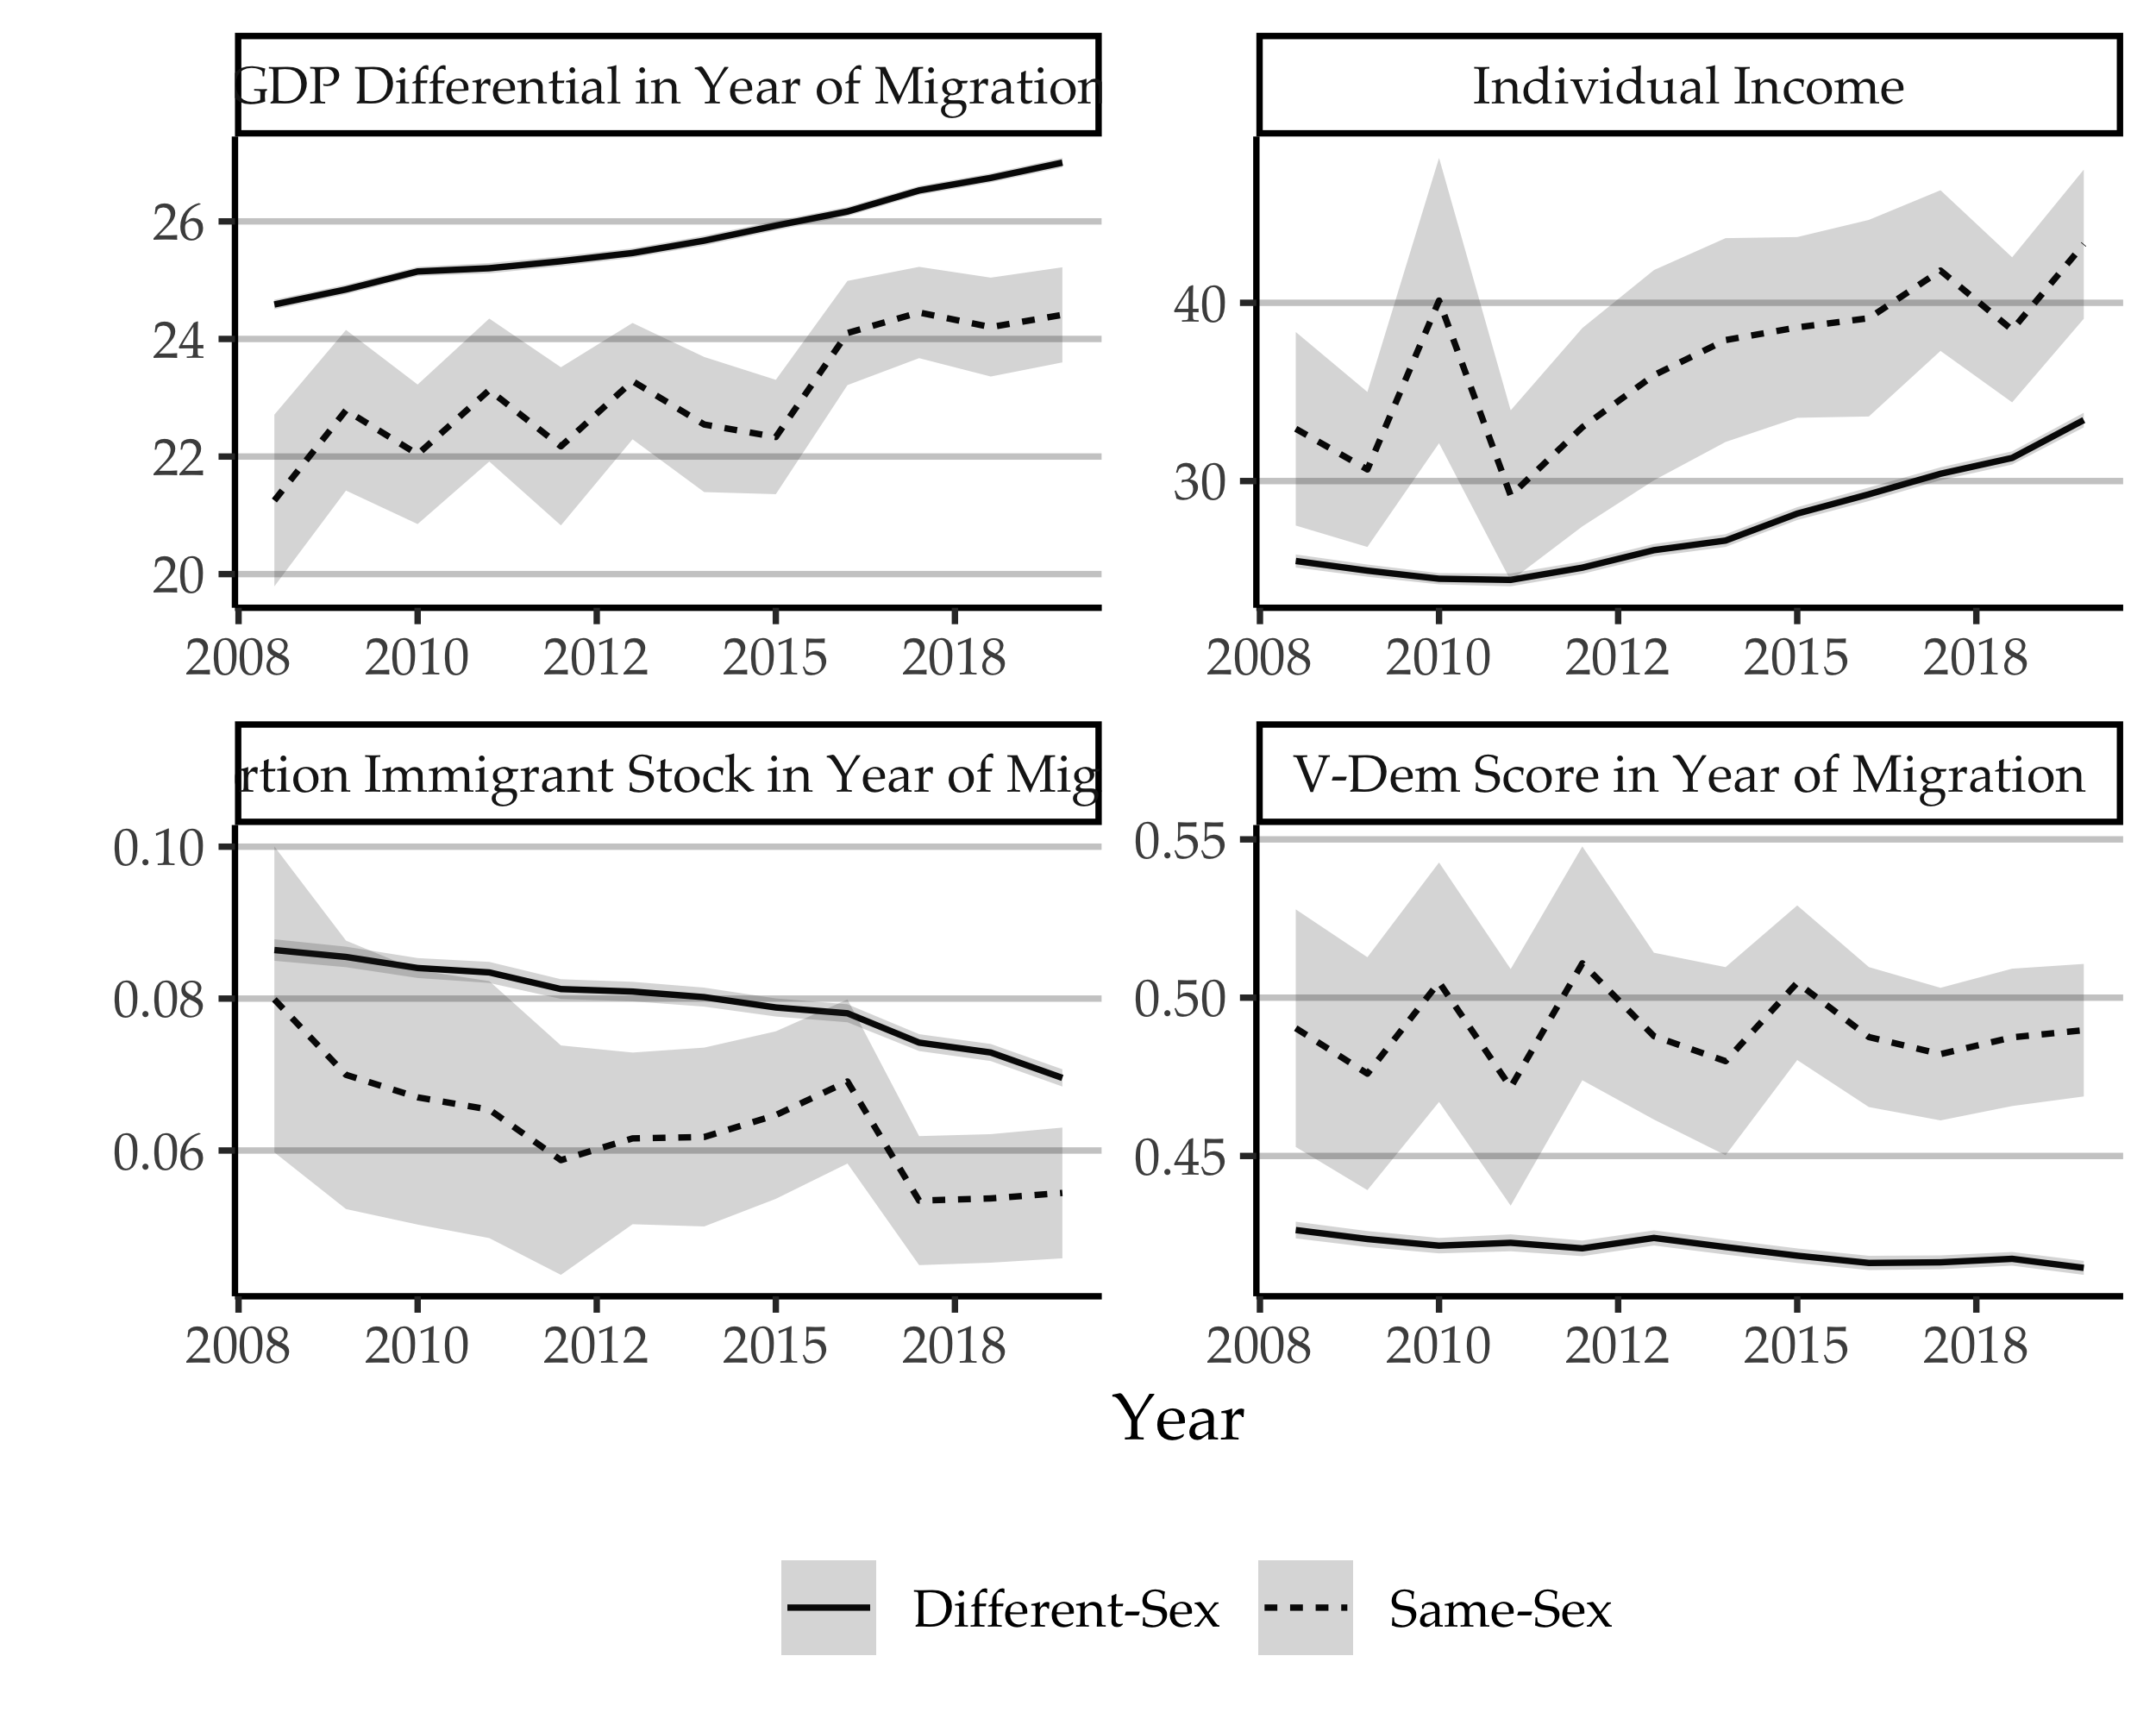
\includegraphics{paa_ssimm_did_files/figure-latex/desc-1.pdf}
\caption{\label{fig:desc}Estimated counts of individuals in mixed-citizenship, same-same couples from the American Community Survey. The ``Repressive'' sample includes only countries with a LGB policy score less than 0, and the ``Progressive'' sample includes only those with a score greater than 3.}
\end{figure}

\hypertarget{background}{%
\section{Background}\label{background}}

blah blah Kris

\hypertarget{data-and-methods}{%
\section{Data and Methods}\label{data-and-methods}}

Due to the large number of 0 counts in our sample, a typical Poisson model is not appropriate. We use quasi-maximum likelihood estimation (QMLE) to identify the effect of DOMA's repeal.

\hypertarget{preliminary-results}{%
\section{Preliminary Results}\label{preliminary-results}}

 
  \providecommand{\huxb}[2]{\arrayrulecolor[RGB]{#1}\global\arrayrulewidth=#2pt}
  \providecommand{\huxvb}[2]{\color[RGB]{#1}\vrule width #2pt}
  \providecommand{\huxtpad}[1]{\rule{0pt}{#1}}
  \providecommand{\huxbpad}[1]{\rule[-#1]{0pt}{#1}}

\begin{table}[ht]
\begin{centerbox}
\begin{threeparttable}
\captionsetup{justification=centering,singlelinecheck=off}
\caption{\label{tab:mod-tab} Quasi-Poisson DDD regressions of counts of 
                        mixed-citizenship same-sex couples}
 \setlength{\tabcolsep}{0pt}
\begin{tabularx}{1\textwidth}{p{0.25\textwidth} p{0.25\textwidth} p{0.25\textwidth} p{0.25\textwidth}}


\hhline{>{\huxb{0, 0, 0}{0.8}}->{\huxb{0, 0, 0}{0.8}}->{\huxb{0, 0, 0}{0.8}}->{\huxb{0, 0, 0}{0.8}}-}
\arrayrulecolor{black}

\multicolumn{1}{!{\huxvb{0, 0, 0}{0}}p{0.25\textwidth}!{\huxvb{0, 0, 0}{0}}}{\hspace{6pt}\parbox[b]{0.25\textwidth-6pt-6pt}{\huxtpad{6pt + 1em}\centering \huxbpad{6pt}}} &
\multicolumn{1}{p{0.25\textwidth}!{\huxvb{0, 0, 0}{0}}}{\hspace{6pt}\parbox[b]{0.25\textwidth-6pt-6pt}{\huxtpad{6pt + 1em}\centering Full sample\huxbpad{6pt}}} &
\multicolumn{1}{p{0.25\textwidth}!{\huxvb{0, 0, 0}{0}}}{\hspace{6pt}\parbox[b]{0.25\textwidth-6pt-6pt}{\huxtpad{6pt + 1em}\centering Repressive\huxbpad{6pt}}} &
\multicolumn{1}{p{0.25\textwidth}!{\huxvb{0, 0, 0}{0}}}{\hspace{6pt}\parbox[b]{0.25\textwidth-6pt-6pt}{\huxtpad{6pt + 1em}\centering Progressive\huxbpad{6pt}}} \tabularnewline[-0.5pt]


\hhline{>{\huxb{255, 255, 255}{0.4}}->{\huxb{0, 0, 0}{0.4}}->{\huxb{0, 0, 0}{0.4}}->{\huxb{0, 0, 0}{0.4}}-}
\arrayrulecolor{black}

\multicolumn{1}{!{\huxvb{0, 0, 0}{0}}p{0.25\textwidth}!{\huxvb{0, 0, 0}{0}}}{\hspace{6pt}\parbox[b]{0.25\textwidth-6pt-6pt}{\huxtpad{6pt + 1em}\raggedright Post-2013 × Same-sex × Mixed-citizenship\huxbpad{6pt}}} &
\multicolumn{1}{p{0.25\textwidth}!{\huxvb{0, 0, 0}{0}}}{\hspace{6pt}\parbox[b]{0.25\textwidth-6pt-6pt}{\huxtpad{6pt + 1em}\raggedleft 0.326 ***\huxbpad{6pt}}} &
\multicolumn{1}{p{0.25\textwidth}!{\huxvb{0, 0, 0}{0}}}{\hspace{6pt}\parbox[b]{0.25\textwidth-6pt-6pt}{\huxtpad{6pt + 1em}\raggedleft 0.061\hphantom{0}\hphantom{0}\hphantom{0}\hphantom{0}\huxbpad{6pt}}} &
\multicolumn{1}{p{0.25\textwidth}!{\huxvb{0, 0, 0}{0}}}{\hspace{6pt}\parbox[b]{0.25\textwidth-6pt-6pt}{\huxtpad{6pt + 1em}\raggedleft 0.415 ***\huxbpad{6pt}}} \tabularnewline[-0.5pt]


\hhline{}
\arrayrulecolor{black}

\multicolumn{1}{!{\huxvb{0, 0, 0}{0}}p{0.25\textwidth}!{\huxvb{0, 0, 0}{0}}}{\hspace{6pt}\parbox[b]{0.25\textwidth-6pt-6pt}{\huxtpad{6pt + 1em}\raggedright \huxbpad{6pt}}} &
\multicolumn{1}{p{0.25\textwidth}!{\huxvb{0, 0, 0}{0}}}{\hspace{6pt}\parbox[b]{0.25\textwidth-6pt-6pt}{\huxtpad{6pt + 1em}\raggedleft (0.050)\hphantom{0}\hphantom{0}\hphantom{0}\huxbpad{6pt}}} &
\multicolumn{1}{p{0.25\textwidth}!{\huxvb{0, 0, 0}{0}}}{\hspace{6pt}\parbox[b]{0.25\textwidth-6pt-6pt}{\huxtpad{6pt + 1em}\raggedleft (0.095)\hphantom{0}\hphantom{0}\hphantom{0}\huxbpad{6pt}}} &
\multicolumn{1}{p{0.25\textwidth}!{\huxvb{0, 0, 0}{0}}}{\hspace{6pt}\parbox[b]{0.25\textwidth-6pt-6pt}{\huxtpad{6pt + 1em}\raggedleft (0.089)\hphantom{0}\hphantom{0}\hphantom{0}\huxbpad{6pt}}} \tabularnewline[-0.5pt]


\hhline{}
\arrayrulecolor{black}

\multicolumn{1}{!{\huxvb{0, 0, 0}{0}}p{0.25\textwidth}!{\huxvb{0, 0, 0}{0}}}{\hspace{6pt}\parbox[b]{0.25\textwidth-6pt-6pt}{\huxtpad{6pt + 1em}\raggedright Post-2013 × Same-sex\huxbpad{6pt}}} &
\multicolumn{1}{p{0.25\textwidth}!{\huxvb{0, 0, 0}{0}}}{\hspace{6pt}\parbox[b]{0.25\textwidth-6pt-6pt}{\huxtpad{6pt + 1em}\raggedleft 0.370 ***\huxbpad{6pt}}} &
\multicolumn{1}{p{0.25\textwidth}!{\huxvb{0, 0, 0}{0}}}{\hspace{6pt}\parbox[b]{0.25\textwidth-6pt-6pt}{\huxtpad{6pt + 1em}\raggedleft 0.374 ***\huxbpad{6pt}}} &
\multicolumn{1}{p{0.25\textwidth}!{\huxvb{0, 0, 0}{0}}}{\hspace{6pt}\parbox[b]{0.25\textwidth-6pt-6pt}{\huxtpad{6pt + 1em}\raggedleft 0.373 ***\huxbpad{6pt}}} \tabularnewline[-0.5pt]


\hhline{}
\arrayrulecolor{black}

\multicolumn{1}{!{\huxvb{0, 0, 0}{0}}p{0.25\textwidth}!{\huxvb{0, 0, 0}{0}}}{\hspace{6pt}\parbox[b]{0.25\textwidth-6pt-6pt}{\huxtpad{6pt + 1em}\raggedright \huxbpad{6pt}}} &
\multicolumn{1}{p{0.25\textwidth}!{\huxvb{0, 0, 0}{0}}}{\hspace{6pt}\parbox[b]{0.25\textwidth-6pt-6pt}{\huxtpad{6pt + 1em}\raggedleft (0.017)\hphantom{0}\hphantom{0}\hphantom{0}\huxbpad{6pt}}} &
\multicolumn{1}{p{0.25\textwidth}!{\huxvb{0, 0, 0}{0}}}{\hspace{6pt}\parbox[b]{0.25\textwidth-6pt-6pt}{\huxtpad{6pt + 1em}\raggedleft (0.019)\hphantom{0}\hphantom{0}\hphantom{0}\huxbpad{6pt}}} &
\multicolumn{1}{p{0.25\textwidth}!{\huxvb{0, 0, 0}{0}}}{\hspace{6pt}\parbox[b]{0.25\textwidth-6pt-6pt}{\huxtpad{6pt + 1em}\raggedleft (0.018)\hphantom{0}\hphantom{0}\hphantom{0}\huxbpad{6pt}}} \tabularnewline[-0.5pt]


\hhline{}
\arrayrulecolor{black}

\multicolumn{1}{!{\huxvb{0, 0, 0}{0}}p{0.25\textwidth}!{\huxvb{0, 0, 0}{0}}}{\hspace{6pt}\parbox[b]{0.25\textwidth-6pt-6pt}{\huxtpad{6pt + 1em}\raggedright Post-2013 × Mixed-citizenship\huxbpad{6pt}}} &
\multicolumn{1}{p{0.25\textwidth}!{\huxvb{0, 0, 0}{0}}}{\hspace{6pt}\parbox[b]{0.25\textwidth-6pt-6pt}{\huxtpad{6pt + 1em}\raggedleft 0.101 ***\huxbpad{6pt}}} &
\multicolumn{1}{p{0.25\textwidth}!{\huxvb{0, 0, 0}{0}}}{\hspace{6pt}\parbox[b]{0.25\textwidth-6pt-6pt}{\huxtpad{6pt + 1em}\raggedleft 0.019\hphantom{0}\hphantom{0}\hphantom{0}\hphantom{0}\huxbpad{6pt}}} &
\multicolumn{1}{p{0.25\textwidth}!{\huxvb{0, 0, 0}{0}}}{\hspace{6pt}\parbox[b]{0.25\textwidth-6pt-6pt}{\huxtpad{6pt + 1em}\raggedleft 0.283 ***\huxbpad{6pt}}} \tabularnewline[-0.5pt]


\hhline{}
\arrayrulecolor{black}

\multicolumn{1}{!{\huxvb{0, 0, 0}{0}}p{0.25\textwidth}!{\huxvb{0, 0, 0}{0}}}{\hspace{6pt}\parbox[b]{0.25\textwidth-6pt-6pt}{\huxtpad{6pt + 1em}\raggedright \huxbpad{6pt}}} &
\multicolumn{1}{p{0.25\textwidth}!{\huxvb{0, 0, 0}{0}}}{\hspace{6pt}\parbox[b]{0.25\textwidth-6pt-6pt}{\huxtpad{6pt + 1em}\raggedleft (0.015)\hphantom{0}\hphantom{0}\hphantom{0}\huxbpad{6pt}}} &
\multicolumn{1}{p{0.25\textwidth}!{\huxvb{0, 0, 0}{0}}}{\hspace{6pt}\parbox[b]{0.25\textwidth-6pt-6pt}{\huxtpad{6pt + 1em}\raggedleft (0.049)\hphantom{0}\hphantom{0}\hphantom{0}\huxbpad{6pt}}} &
\multicolumn{1}{p{0.25\textwidth}!{\huxvb{0, 0, 0}{0}}}{\hspace{6pt}\parbox[b]{0.25\textwidth-6pt-6pt}{\huxtpad{6pt + 1em}\raggedleft (0.042)\hphantom{0}\hphantom{0}\hphantom{0}\huxbpad{6pt}}} \tabularnewline[-0.5pt]


\hhline{}
\arrayrulecolor{black}

\multicolumn{1}{!{\huxvb{0, 0, 0}{0}}p{0.25\textwidth}!{\huxvb{0, 0, 0}{0}}}{\hspace{6pt}\parbox[b]{0.25\textwidth-6pt-6pt}{\huxtpad{6pt + 1em}\raggedright Post-2013\huxbpad{6pt}}} &
\multicolumn{1}{p{0.25\textwidth}!{\huxvb{0, 0, 0}{0}}}{\hspace{6pt}\parbox[b]{0.25\textwidth-6pt-6pt}{\huxtpad{6pt + 1em}\raggedleft -0.035 **\hphantom{0}\huxbpad{6pt}}} &
\multicolumn{1}{p{0.25\textwidth}!{\huxvb{0, 0, 0}{0}}}{\hspace{6pt}\parbox[b]{0.25\textwidth-6pt-6pt}{\huxtpad{6pt + 1em}\raggedleft -0.065 ***\huxbpad{6pt}}} &
\multicolumn{1}{p{0.25\textwidth}!{\huxvb{0, 0, 0}{0}}}{\hspace{6pt}\parbox[b]{0.25\textwidth-6pt-6pt}{\huxtpad{6pt + 1em}\raggedleft -0.038 *\hphantom{0}\hphantom{0}\huxbpad{6pt}}} \tabularnewline[-0.5pt]


\hhline{}
\arrayrulecolor{black}

\multicolumn{1}{!{\huxvb{0, 0, 0}{0}}p{0.25\textwidth}!{\huxvb{0, 0, 0}{0}}}{\hspace{6pt}\parbox[b]{0.25\textwidth-6pt-6pt}{\huxtpad{6pt + 1em}\raggedright \huxbpad{6pt}}} &
\multicolumn{1}{p{0.25\textwidth}!{\huxvb{0, 0, 0}{0}}}{\hspace{6pt}\parbox[b]{0.25\textwidth-6pt-6pt}{\huxtpad{6pt + 1em}\raggedleft (0.011)\hphantom{0}\hphantom{0}\hphantom{0}\huxbpad{6pt}}} &
\multicolumn{1}{p{0.25\textwidth}!{\huxvb{0, 0, 0}{0}}}{\hspace{6pt}\parbox[b]{0.25\textwidth-6pt-6pt}{\huxtpad{6pt + 1em}\raggedleft (0.011)\hphantom{0}\hphantom{0}\hphantom{0}\huxbpad{6pt}}} &
\multicolumn{1}{p{0.25\textwidth}!{\huxvb{0, 0, 0}{0}}}{\hspace{6pt}\parbox[b]{0.25\textwidth-6pt-6pt}{\huxtpad{6pt + 1em}\raggedleft (0.015)\hphantom{0}\hphantom{0}\hphantom{0}\huxbpad{6pt}}} \tabularnewline[-0.5pt]


\hhline{>{\huxb{255, 255, 255}{0.4}}->{\huxb{0, 0, 0}{0.4}}->{\huxb{0, 0, 0}{0.4}}->{\huxb{0, 0, 0}{0.4}}-}
\arrayrulecolor{black}

\multicolumn{1}{!{\huxvb{0, 0, 0}{0}}p{0.25\textwidth}!{\huxvb{0, 0, 0}{0}}}{\hspace{6pt}\parbox[b]{0.25\textwidth-6pt-6pt}{\huxtpad{6pt + 1em}\raggedright Observations\huxbpad{6pt}}} &
\multicolumn{1}{p{0.25\textwidth}!{\huxvb{0, 0, 0}{0}}}{\hspace{6pt}\parbox[b]{0.25\textwidth-6pt-6pt}{\huxtpad{6pt + 1em}\raggedleft 2448\hphantom{0}\hphantom{0}\hphantom{0}\hphantom{0}\hphantom{0}\hphantom{0}\hphantom{0}\hphantom{0}\huxbpad{6pt}}} &
\multicolumn{1}{p{0.25\textwidth}!{\huxvb{0, 0, 0}{0}}}{\hspace{6pt}\parbox[b]{0.25\textwidth-6pt-6pt}{\huxtpad{6pt + 1em}\raggedleft 2267\hphantom{0}\hphantom{0}\hphantom{0}\hphantom{0}\hphantom{0}\hphantom{0}\hphantom{0}\hphantom{0}\huxbpad{6pt}}} &
\multicolumn{1}{p{0.25\textwidth}!{\huxvb{0, 0, 0}{0}}}{\hspace{6pt}\parbox[b]{0.25\textwidth-6pt-6pt}{\huxtpad{6pt + 1em}\raggedleft 2345\hphantom{0}\hphantom{0}\hphantom{0}\hphantom{0}\hphantom{0}\hphantom{0}\hphantom{0}\hphantom{0}\huxbpad{6pt}}} \tabularnewline[-0.5pt]


\hhline{>{\huxb{0, 0, 0}{0.8}}->{\huxb{0, 0, 0}{0.8}}->{\huxb{0, 0, 0}{0.8}}->{\huxb{0, 0, 0}{0.8}}-}
\arrayrulecolor{black}

\multicolumn{4}{!{\huxvb{0, 0, 0}{0}}p{1\textwidth+6\tabcolsep}!{\huxvb{0, 0, 0}{0}}}{\hspace{6pt}\parbox[b]{1\textwidth+6\tabcolsep-6pt-6pt}{\huxtpad{6pt + 1em}\raggedright  *** p $<$ 0.001;  ** p $<$ 0.01;  * p $<$ 0.05;  † p $<$ 0.1. The "Repressive" sample includes only countries with a LGB policy score less than 0, and the "Progressive" sample includes only those with a score greater than 3. Group-clustered standard errors shown in parentheses. Source: American Community Survey 2008-2019.\huxbpad{6pt}}} \tabularnewline[-0.5pt]


\hhline{}
\arrayrulecolor{black}
\end{tabularx}
\end{threeparttable}\par\end{centerbox}

\end{table}
 

Table \ref{tab:mod-tab} presents results from our DDD specifications. For the full sample, the incidence of individuals in mixed-citizenship, same-sex couples grew by \(100 \times [\exp(0.33) -1] =\) 38 percent after 2013, relative to those in couples that were not same-sex or mixed-citizenship.

\begin{figure}
\centering
\includegraphics{paa_ssimm_did_files/figure-latex/lag-plot-1.pdf}
\caption{\label{fig:lag-plot}Lag-lead specification of quasi-poisson TWFE DDD regression}
\end{figure}

\newpage

\hypertarget{appendix}{%
\section{Appendix}\label{appendix}}

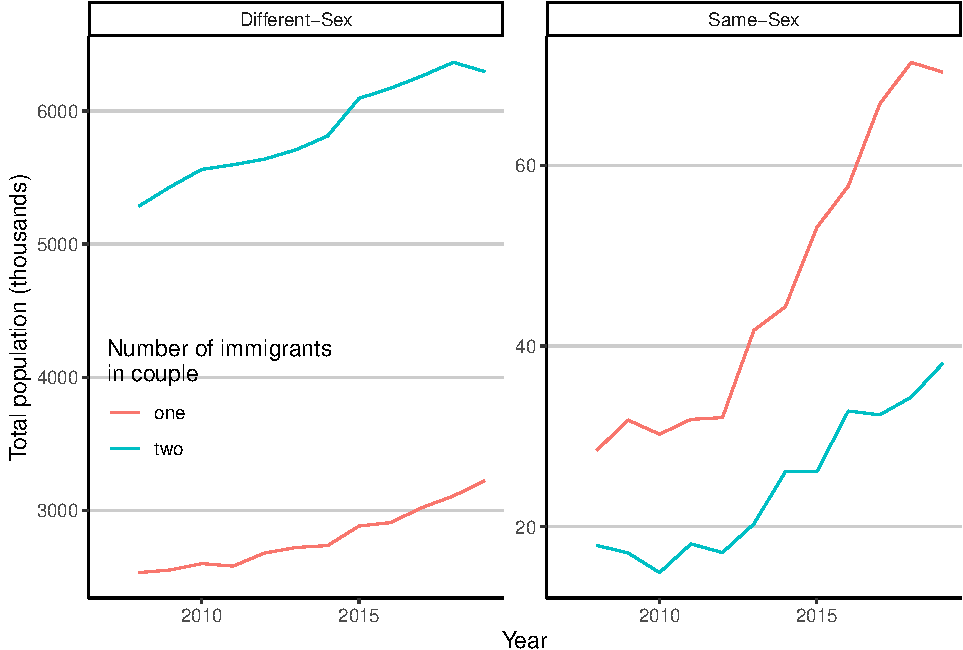
\includegraphics{paa_ssimm_did_files/figure-latex/unnamed-chunk-1-1.pdf}

\end{document}
